\documentclass[11pt]{article}
\usepackage[margin=1in]{geometry}

\usepackage{amsmath}
\usepackage{amssymb}
\usepackage[utf8]{inputenc} 
\usepackage{graphicx} 
\usepackage{parskip} 
\usepackage{multirow} 
\usepackage{mathtools}

\DeclarePairedDelimiter\abs{\lvert}{\rvert}%
\DeclarePairedDelimiter\norm{\lVert}{\rVert}%

\makeatletter
\let\oldabs\abs
\def\abs{\@ifstar{\oldabs}{\oldabs*}}

\let\oldnorm\norm
\def\norm{\@ifstar{\oldnorm}{\oldnorm*}}
\makeatother
\usepackage{multicol} 
\usepackage[spanish,es-nodecimaldot]{babel} 
\usepackage{mathtools}
\usepackage{amsfonts}
\usepackage{float}
\usepackage{textcomp}
\usepackage{caption}
\usepackage{subfig}
\usepackage[spanish]{babel}
\usepackage{gensymb}
\def\sen{\mathop{\mbox{\normalfont sen}}\nolimits}

\usepackage{fancyhdr}
\fancyhf{}
\rfoot{\thepage}
\pagestyle{fancy}
\lhead{Nieto Castellanos Jaime Fabián}
\chead{}
\rhead{Tarea 8. Histogramas}
\begin{document}

\textbf{1)}
\begin{figure}[H]
\centering
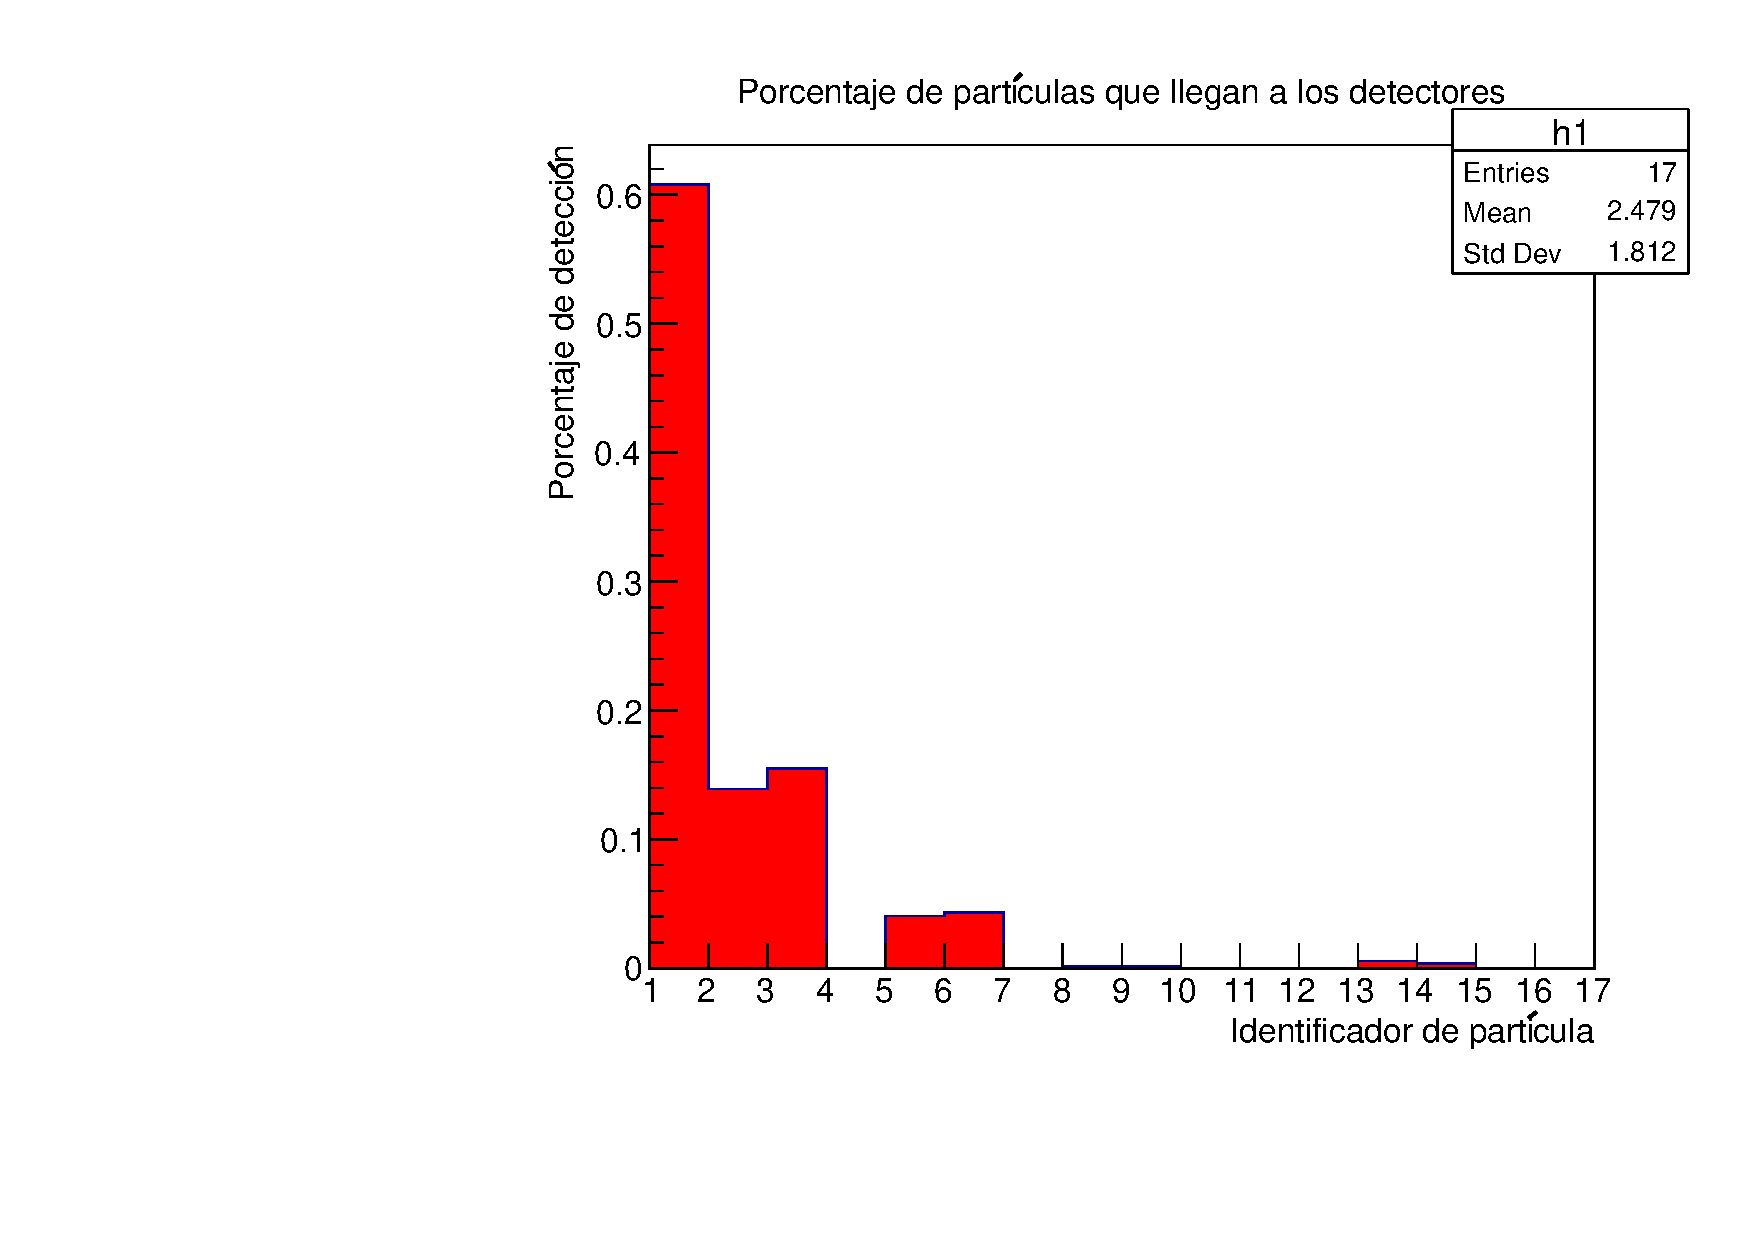
\includegraphics[width=0.7\textwidth]{../Figuras/Prob1A.pdf}
\caption{ Porcentaje de cada tipo de partícula que llega a los detectores de HAWC. El 1 significa $\gamma$, el 2 $e^+$ y el 3 $e^-$}
\label{fig:Prob1A}
\end{figure}
Para separar el conjunto de datos en tres rangos energéticos, lo haremos considerando la integral de la distribución de energía, figura \ref{fig:Prob1B}. Si el área debajo del histograma es $A$, entonces el primer rango de energías corresponde a la primera tercera parte del área, el segundo rango corresponde a la segunda tercera parte del área y el tercer rango corresponde a la última. Los detalles se encuentran en el archivo Prob1.C. Después de realizar el procedimiento anterior, los rangos en los que dividimos nuestro conjunto de datos son [0,2500GeV), [2500GeV,8500GeV) y [8500GeV, 1e5 GeV]. En la figura \ref{fig:Prob1C} se observa que el resultado es prácticamente el mismo en los tres rangos energéticos.


\begin{figure}[H]
\centering
{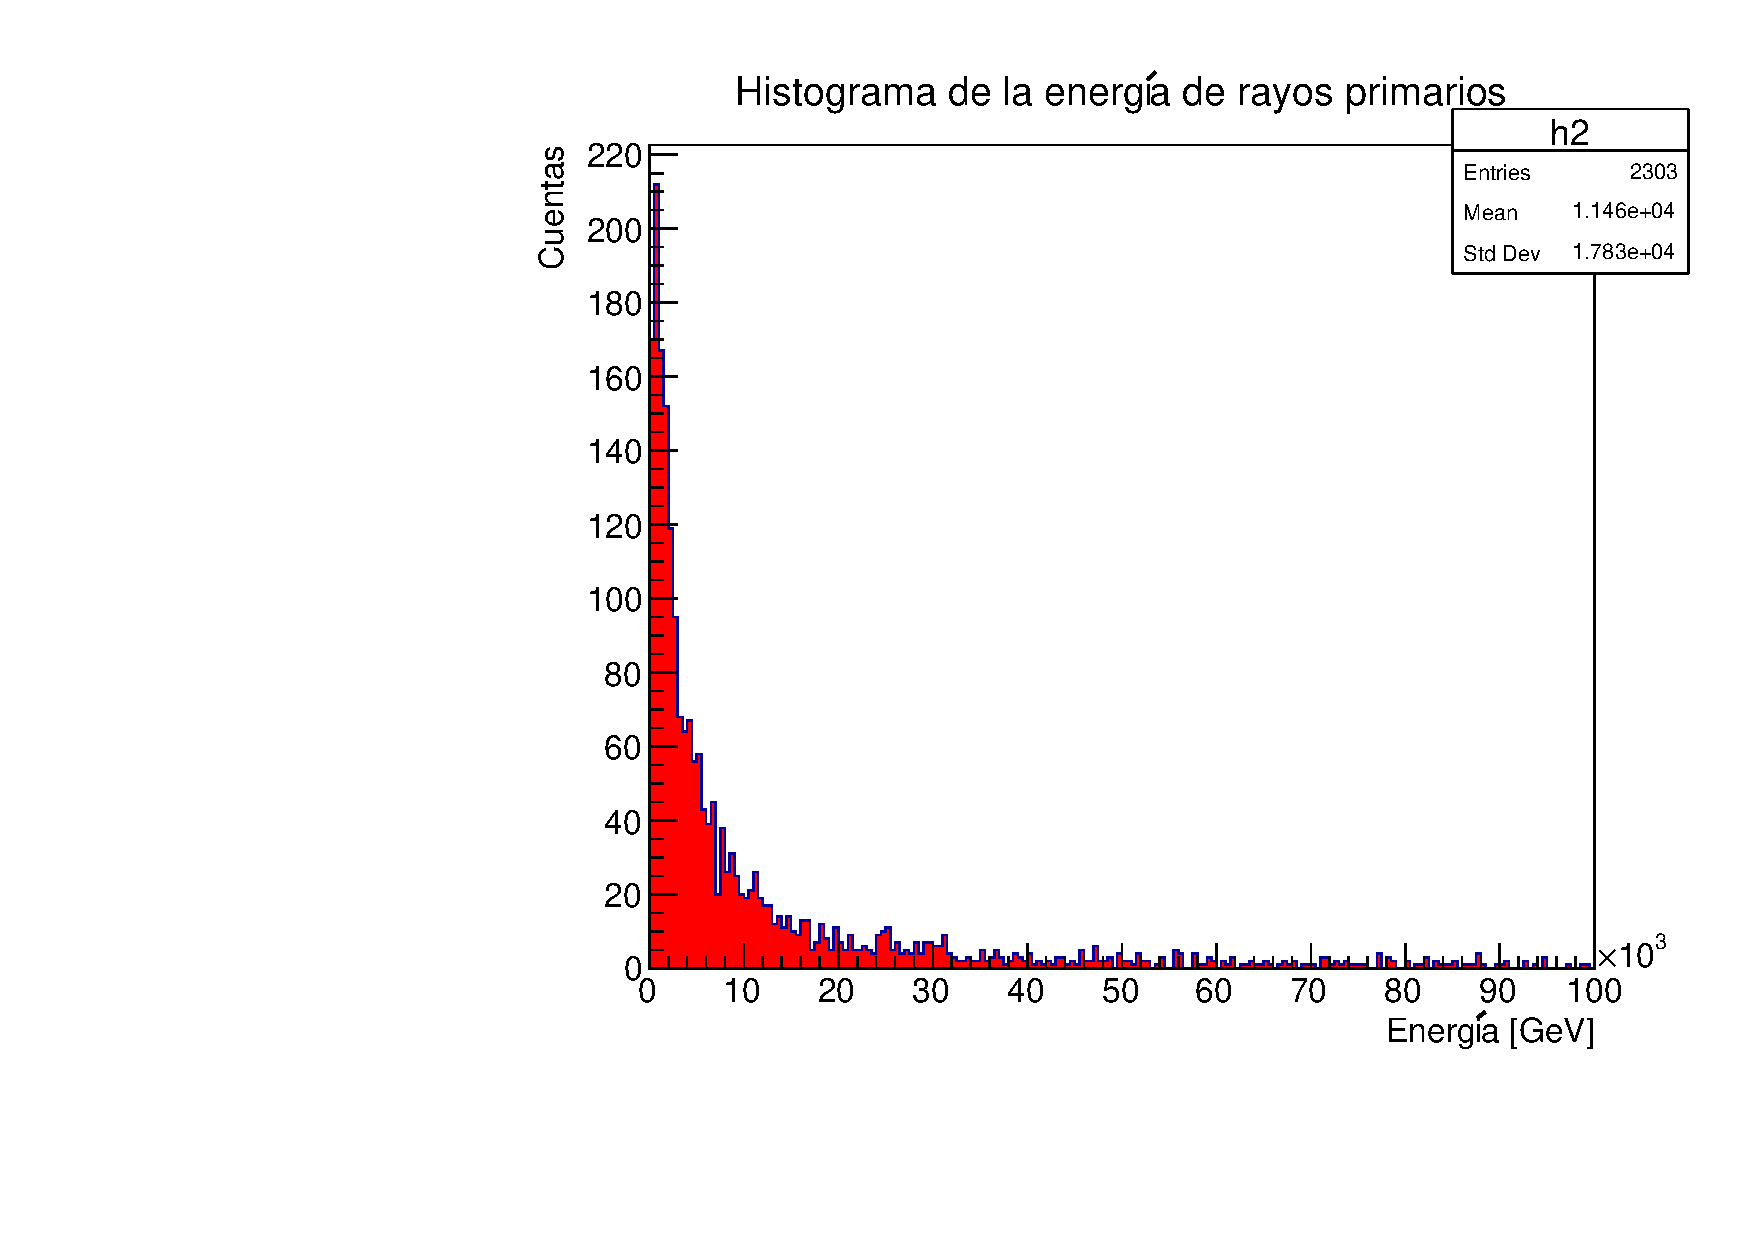
\includegraphics[width=0.7\textwidth]{../Figuras/Prob1B.pdf}}
\caption{ Histograma de la distribución de energía del archivo de datos.}
\label{fig:Prob1B}
\end{figure}


\begin{figure}[H]
\centering
\subfloat[\centering Intervalo [0,2500GeV)]{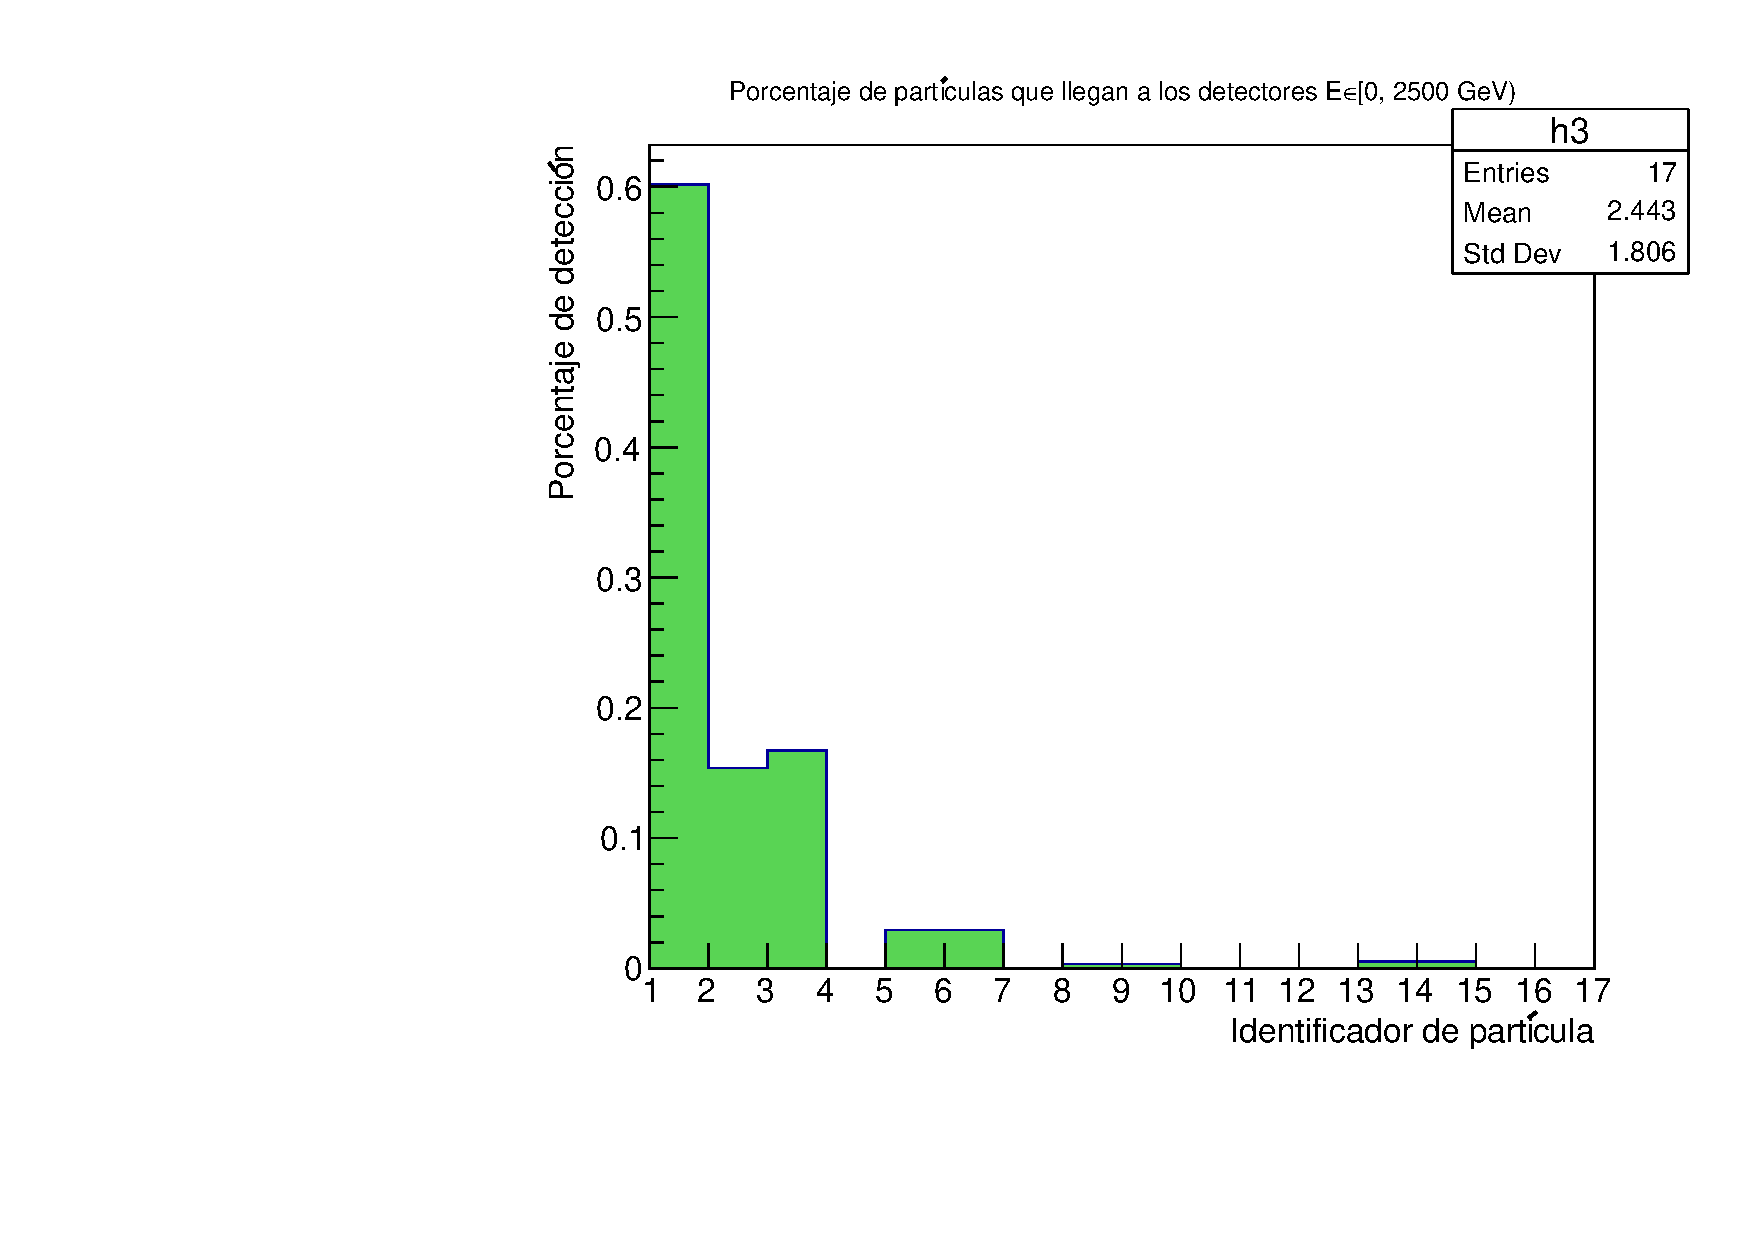
\includegraphics[width=0.7\textwidth]{../Figuras/Prob1C1.pdf}}
\end{figure}

\begin{figure}[H]
\centering
\subfloat[\centering Intervalo [2500GeV,8500GeV)]{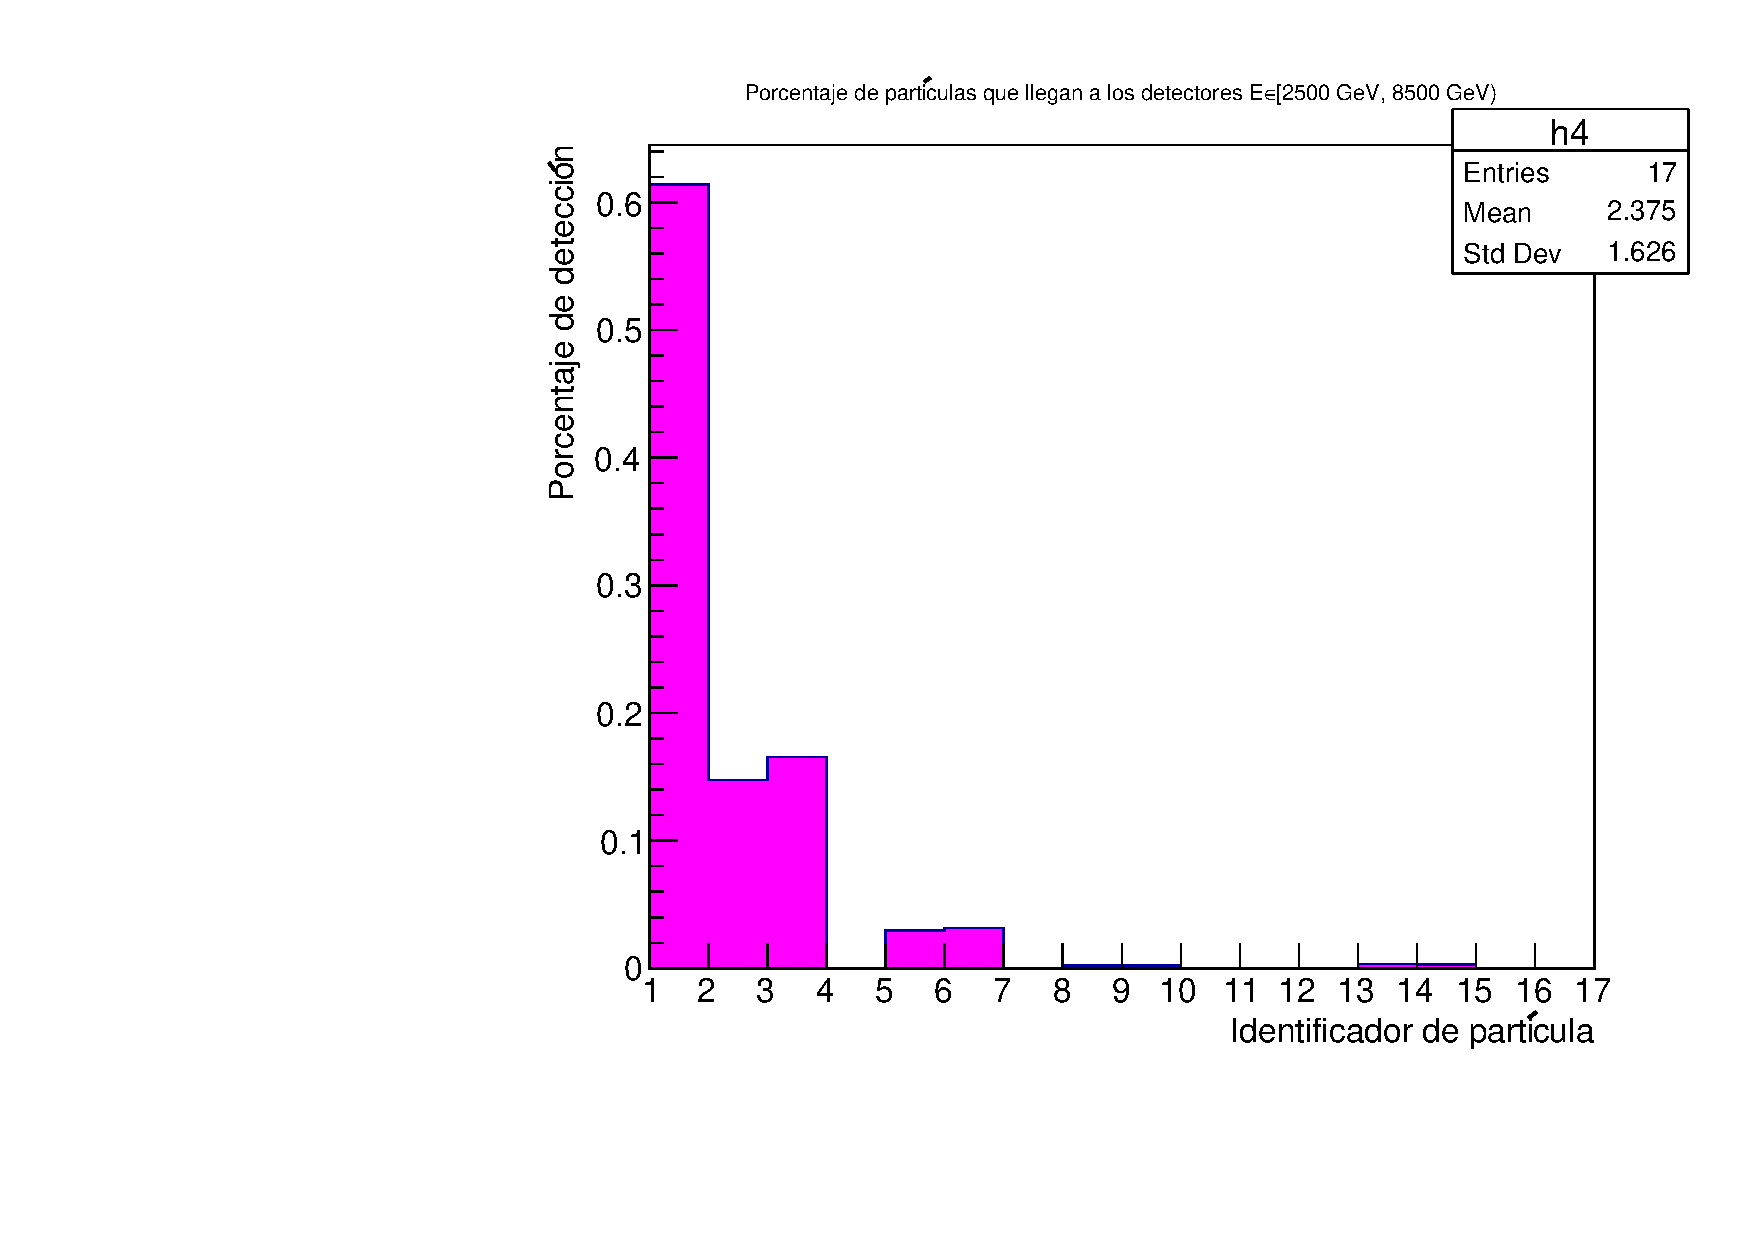
\includegraphics[width=0.7\textwidth]{../Figuras/Prob1C2.pdf}}

\subfloat[\centering Intervalo [8500GeV, 1e5 GeV)]{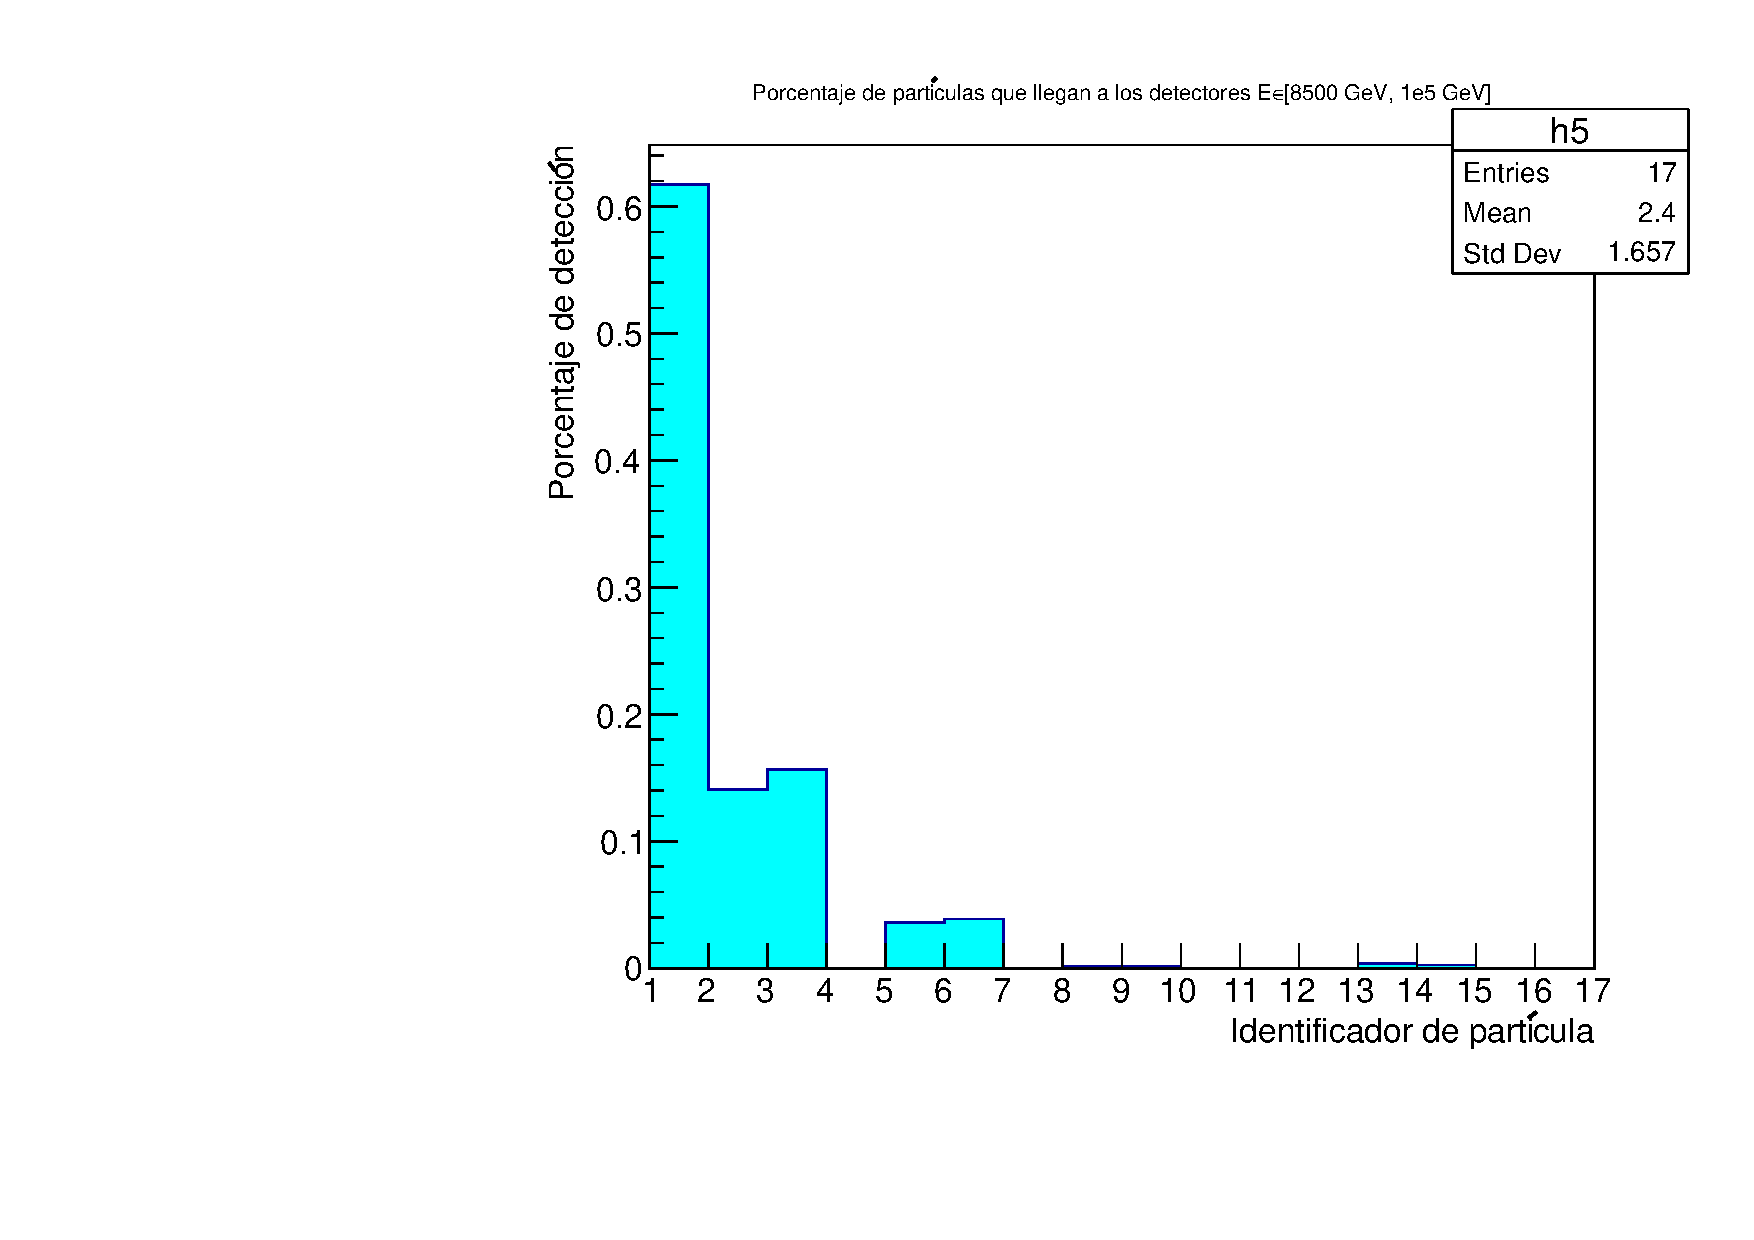
\includegraphics[width=0.7\textwidth]{../Figuras/Prob1C3.pdf}}
\caption{Porcentaje de partículas de cada tipo que llega a los detectores de HAWC para diferentes rangos energéticos con el mismo número de estadística.}
\label{fig:Prob1C}
\end{figure}
\pagebreak
%%%%%%%%%%%%%%%%%%%%%%%%%%%%%%%%%%%%%%%%%%%%%%%%
\textbf{2)} Mostramos la distribución lateral para los eventos 1, 25 y 198.
\begin{figure}[H]
\centering
\subfloat[\centering Evento 1]{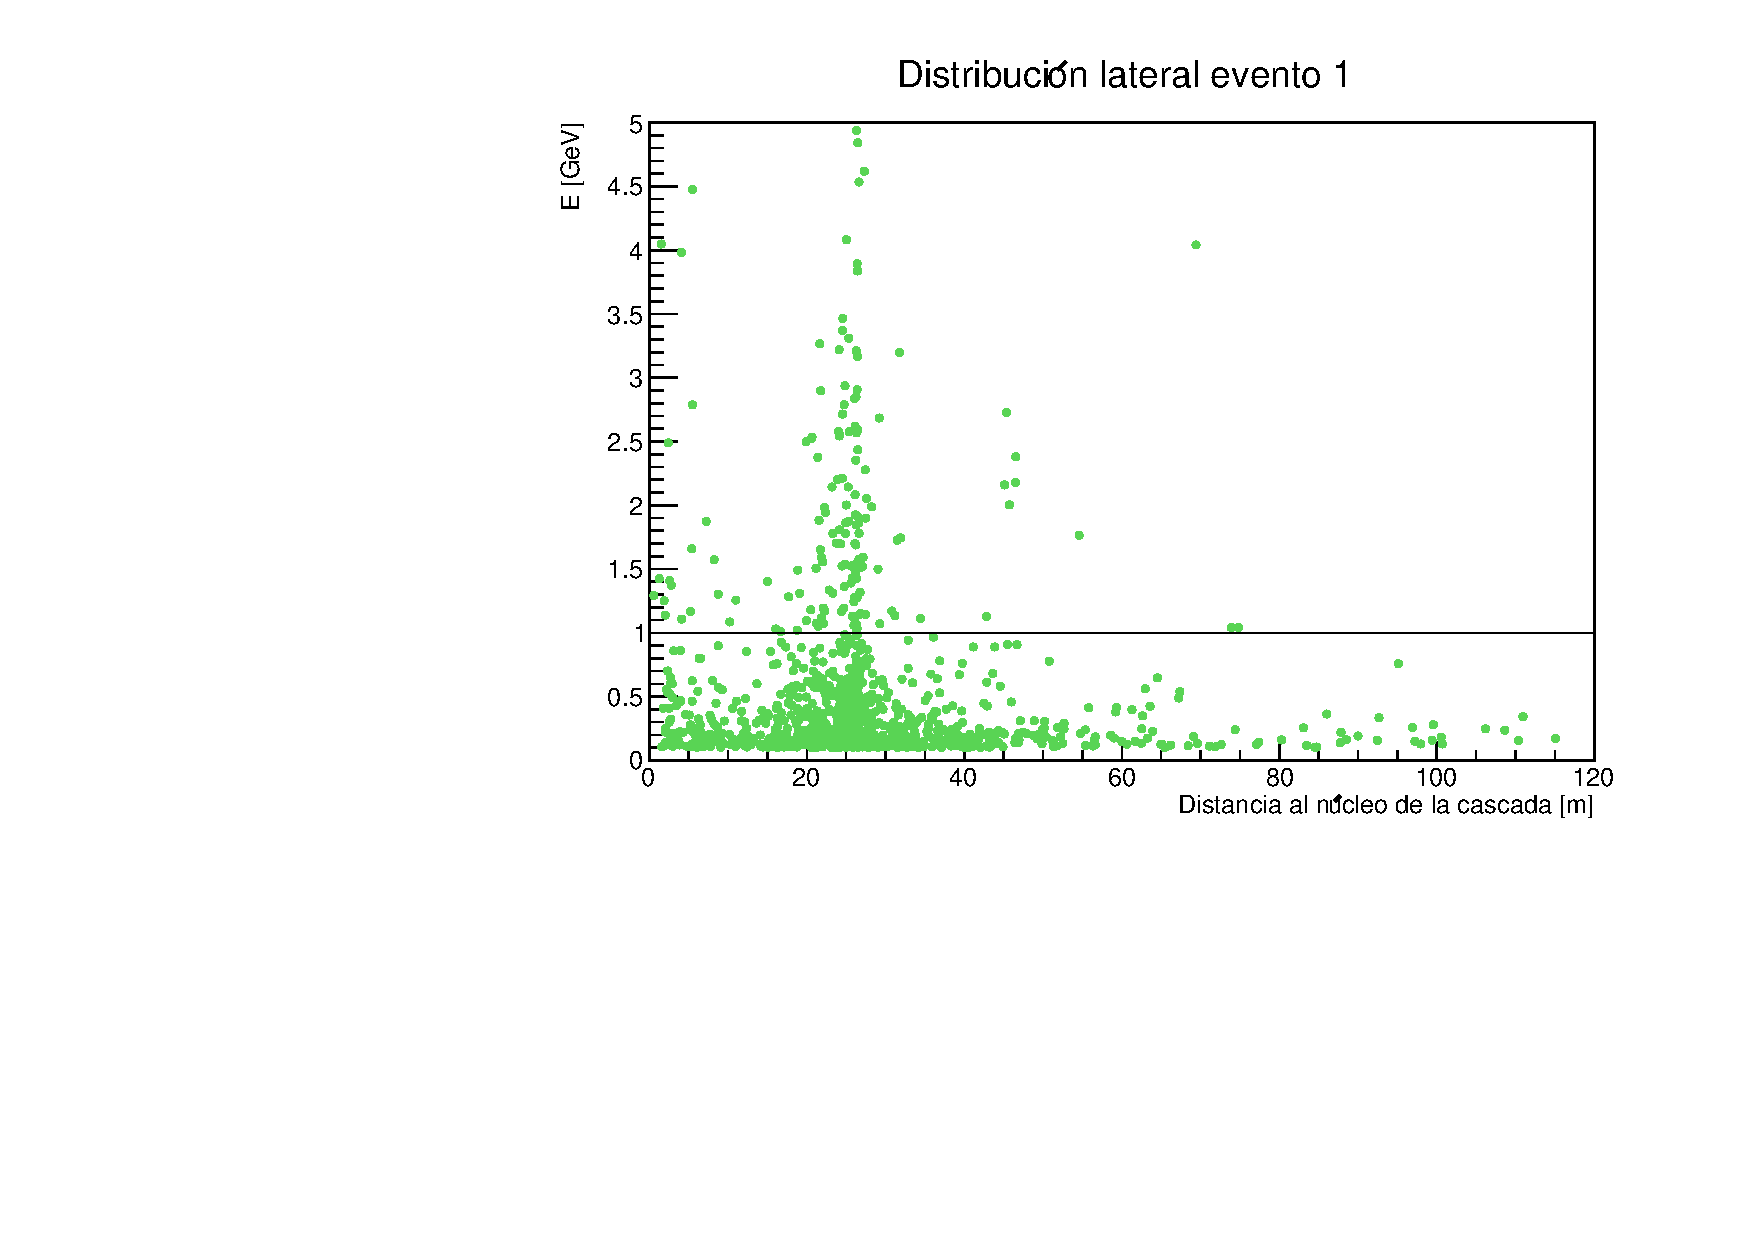
\includegraphics[width=0.9\textwidth]{../Figuras/Prob2A.pdf}}

\subfloat[\centering Evento 25]{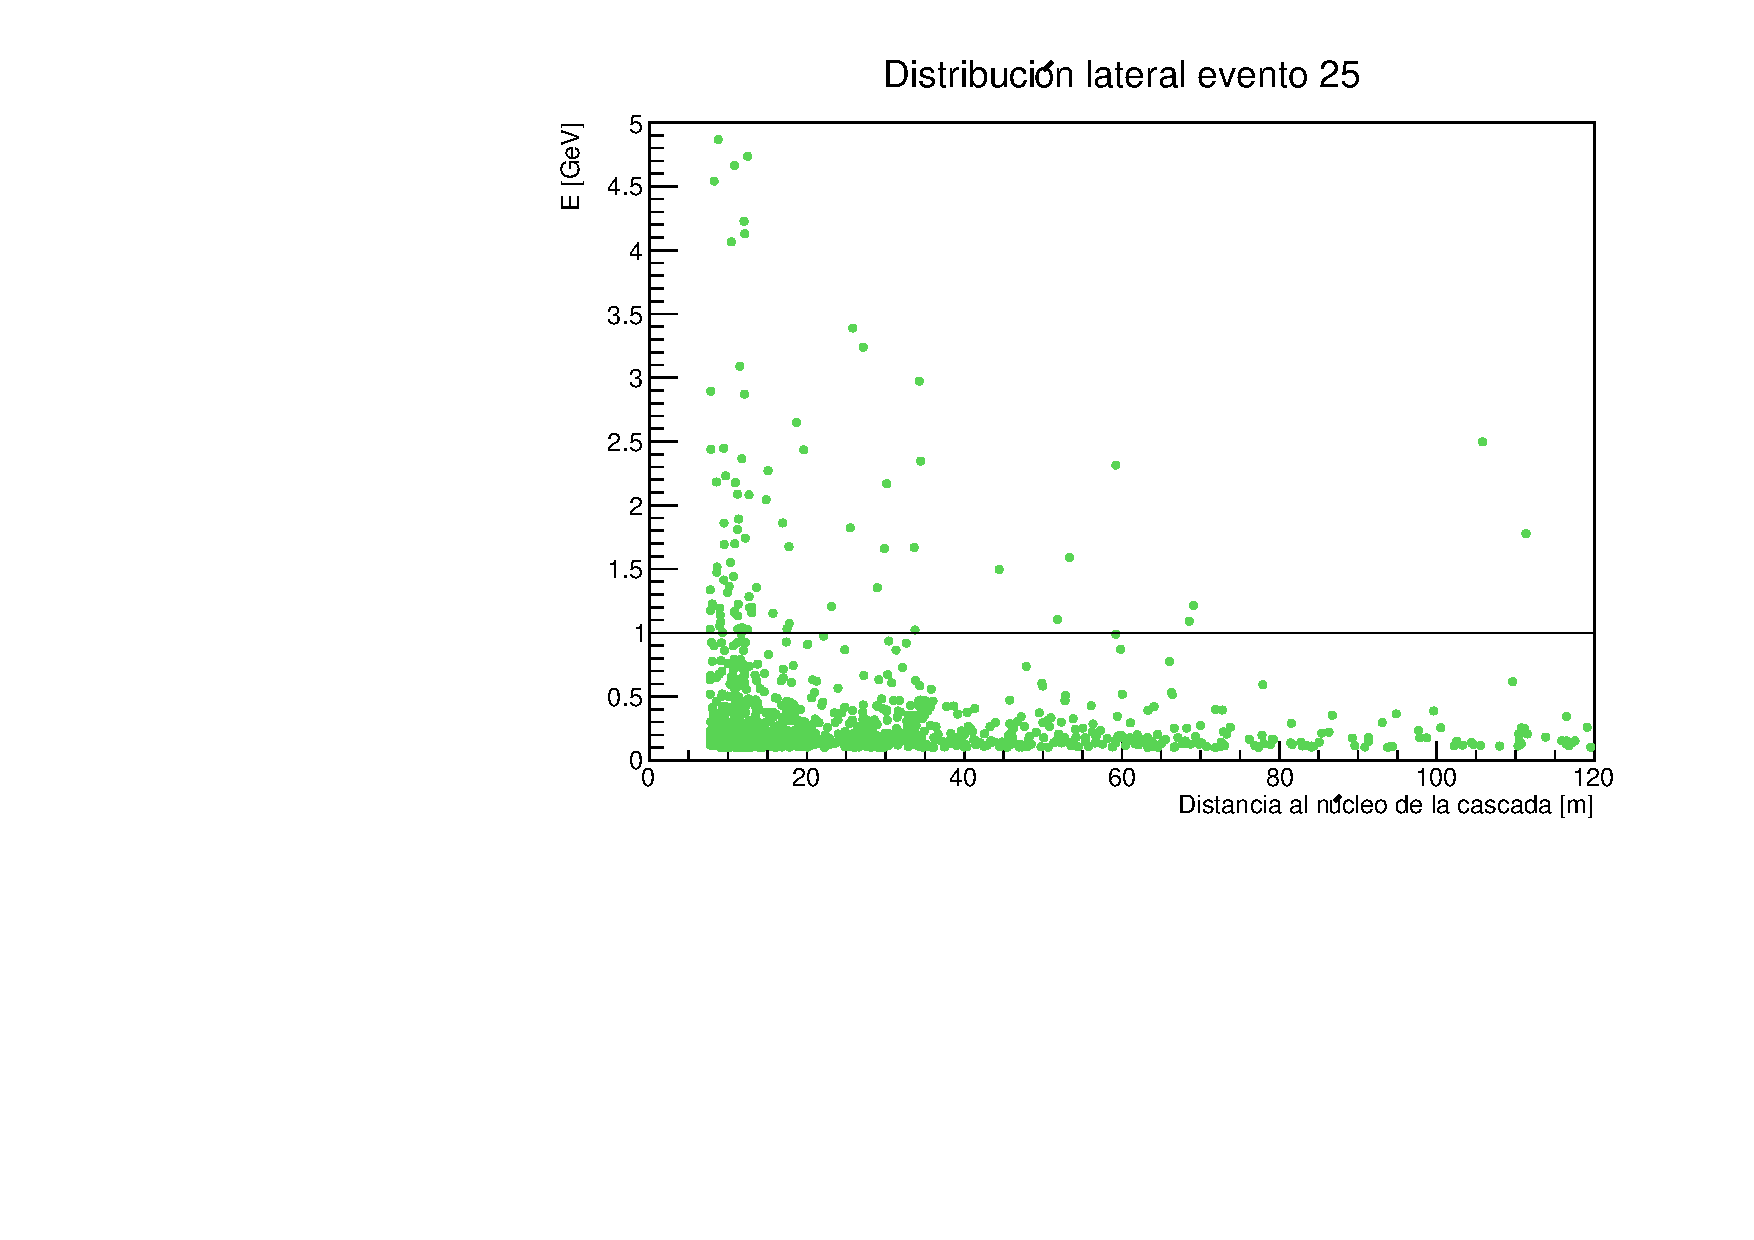
\includegraphics[width=0.9\textwidth]{../Figuras/Prob2B.pdf}}
\end{figure}

\begin{figure}[H]
\centering 
\subfloat[\centering Evento 198]{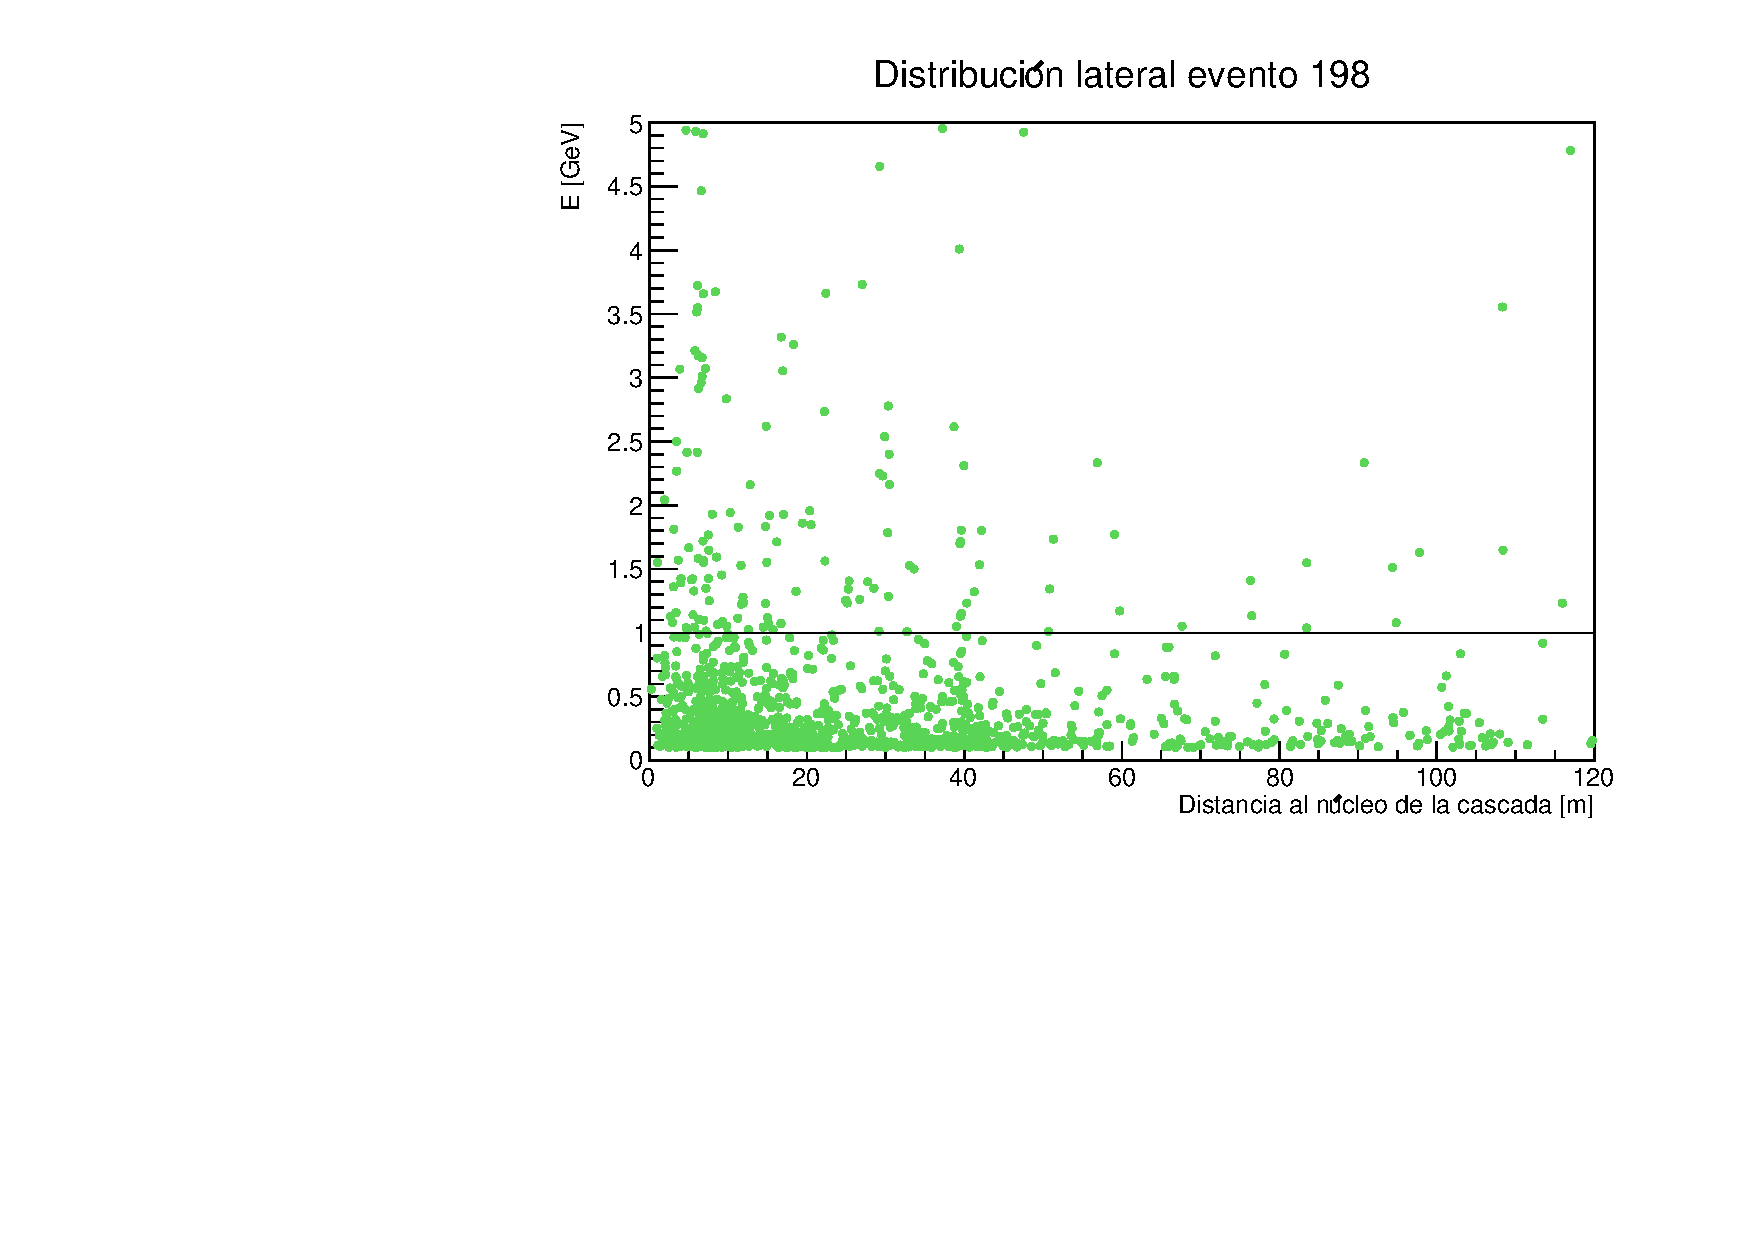
\includegraphics[width=0.9\textwidth]{../Figuras/Prob2C.pdf}}
\caption{Distribución lateral para distintos eventos. Estos eventos satisfacen tener más de 70 hits con un mínimo de 70 GeV.}
\label{fig:Prob2A}
\end{figure}
De los eventos anteriores elegimos el evento 198 para separar la distribución lateral para las tres partículas más abundantes que llegan a los detectores. El resultado se muestra en la figura \ref{fig:Prob2B}.
\begin{figure}[H]
\centering
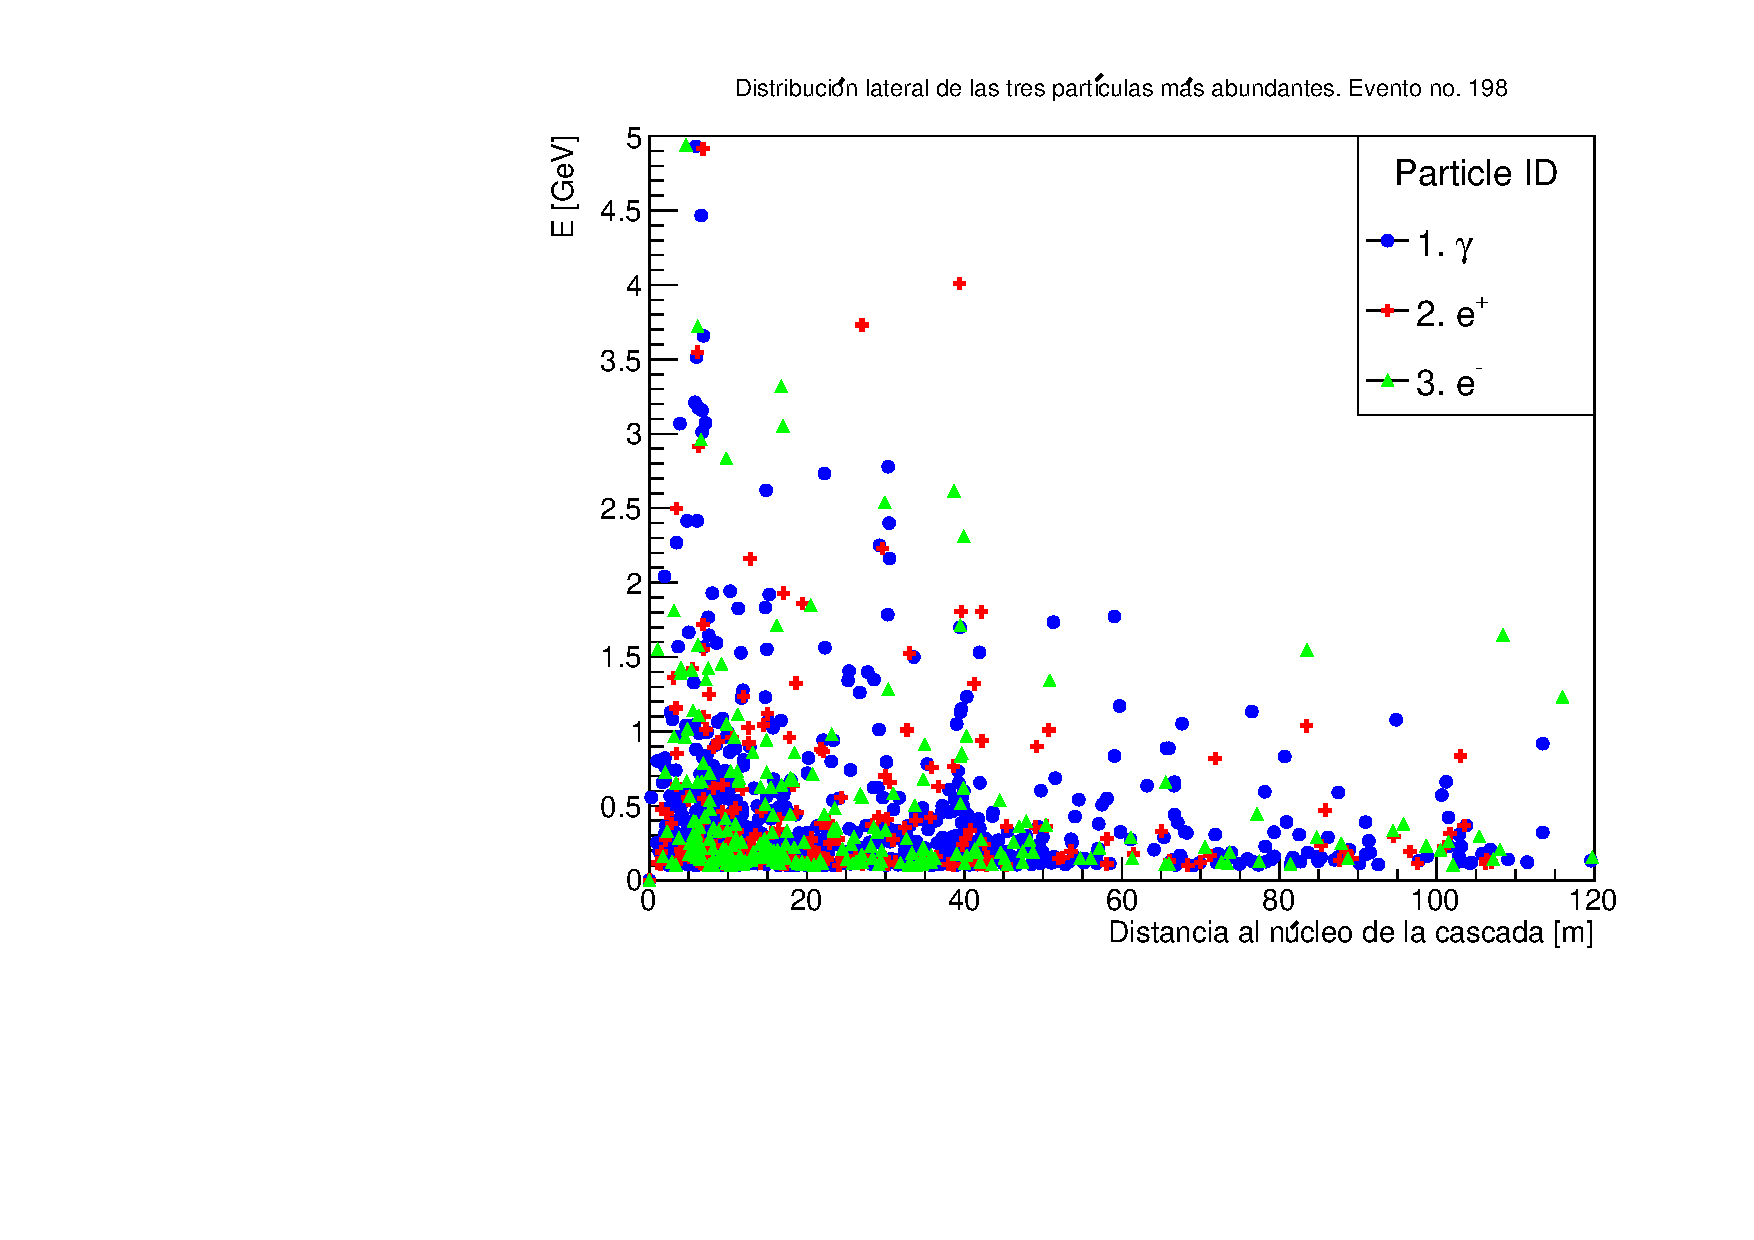
\includegraphics[width=0.9\textwidth]{../Figuras/Prob2D.pdf}
\caption{Distribución lateral para las tres partículas más abundantes, evento 198.}
\label{fig:Prob2B}
\end{figure}
\pagebreak
%%%%%%%%%%%%%%%%%%%%%%%%%%%%%%%%%%%%%%%%%%%%%%%%
\textbf{3)}
\begin{figure}[H]
\centering
\subfloat[\centering Distribución angular $\theta$]{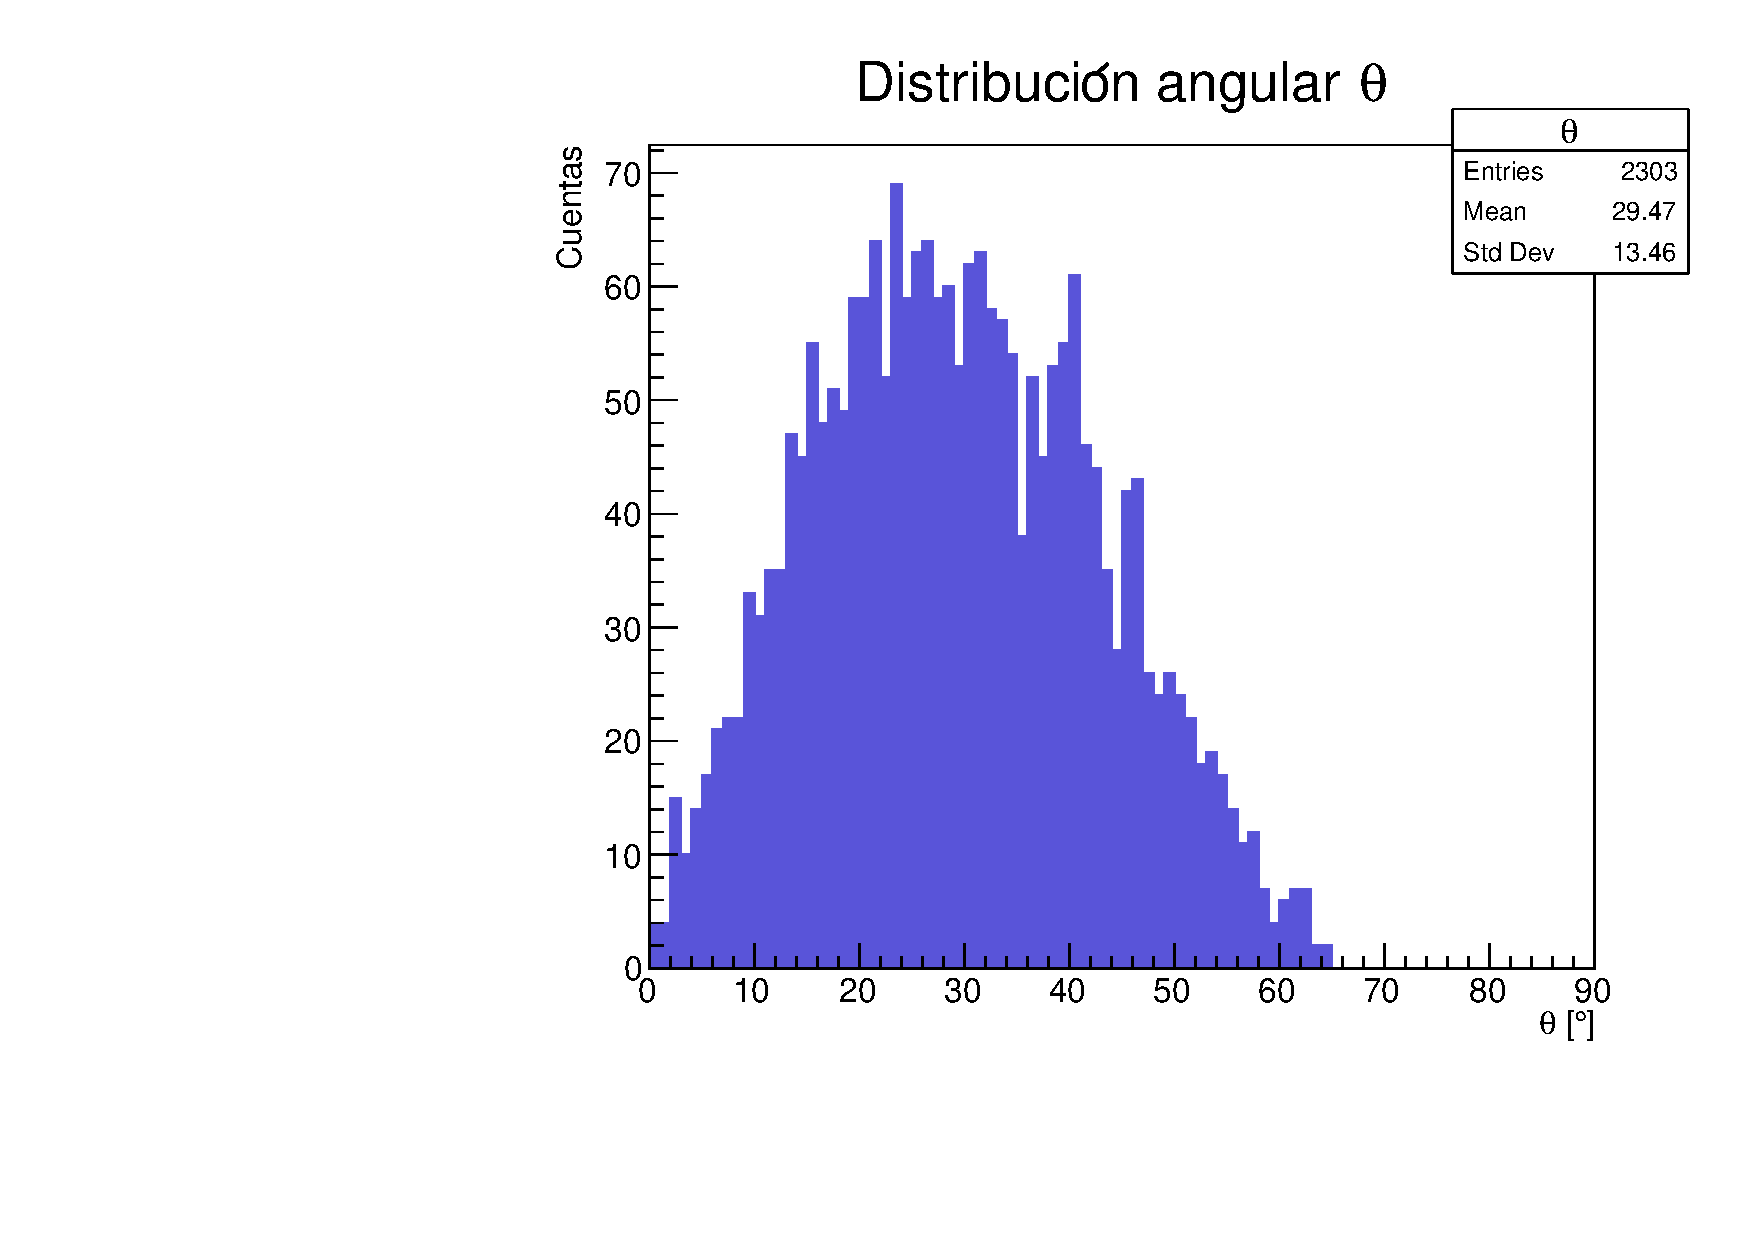
\includegraphics[width=0.68\textwidth]{../Figuras/Prob3A.pdf}}

\subfloat[\centering Distribución angular $\phi$]{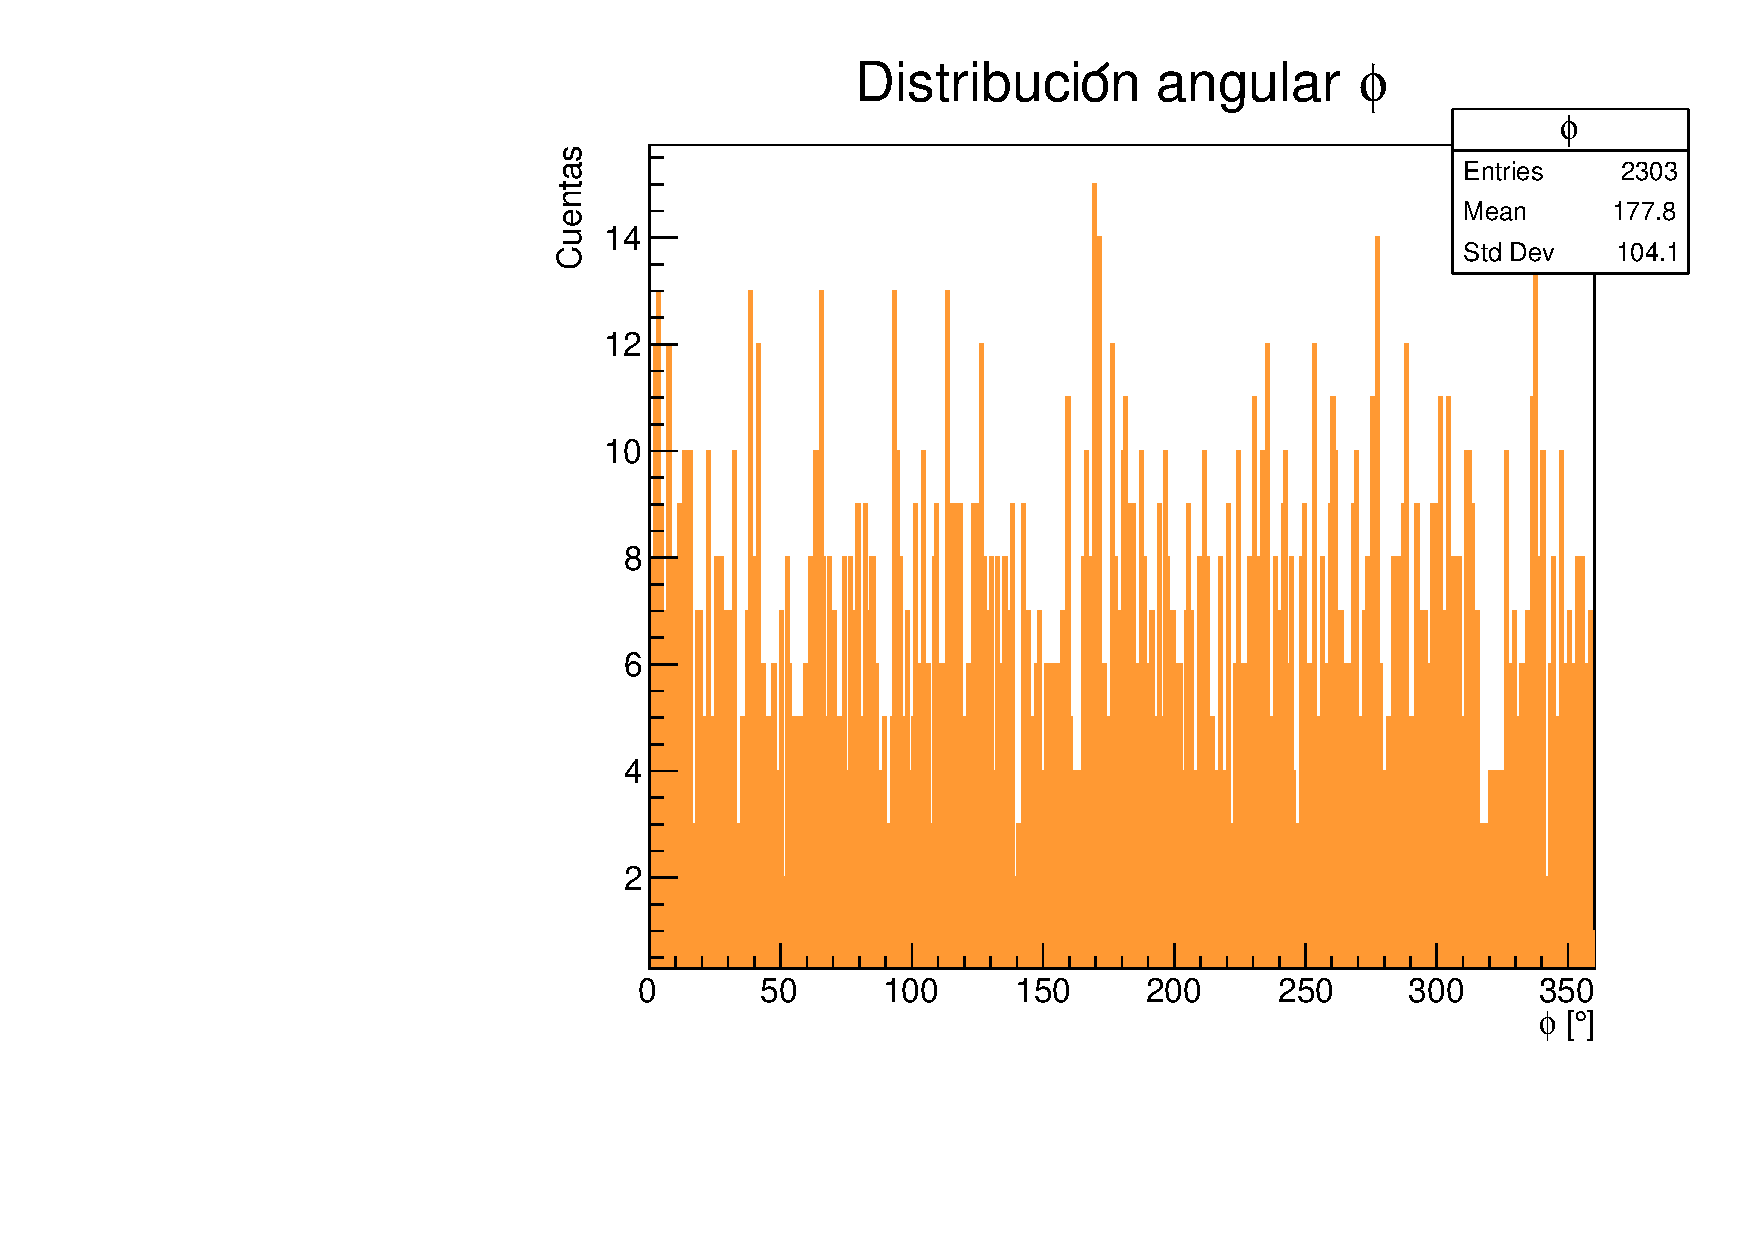
\includegraphics[width=0.68\textwidth]{../Figuras/Prob3B.pdf}}
\caption{Distribuciones angulares}
\end{figure}
\pagebreak

\textbf{4)}
\begin{figure}[H]
\centering
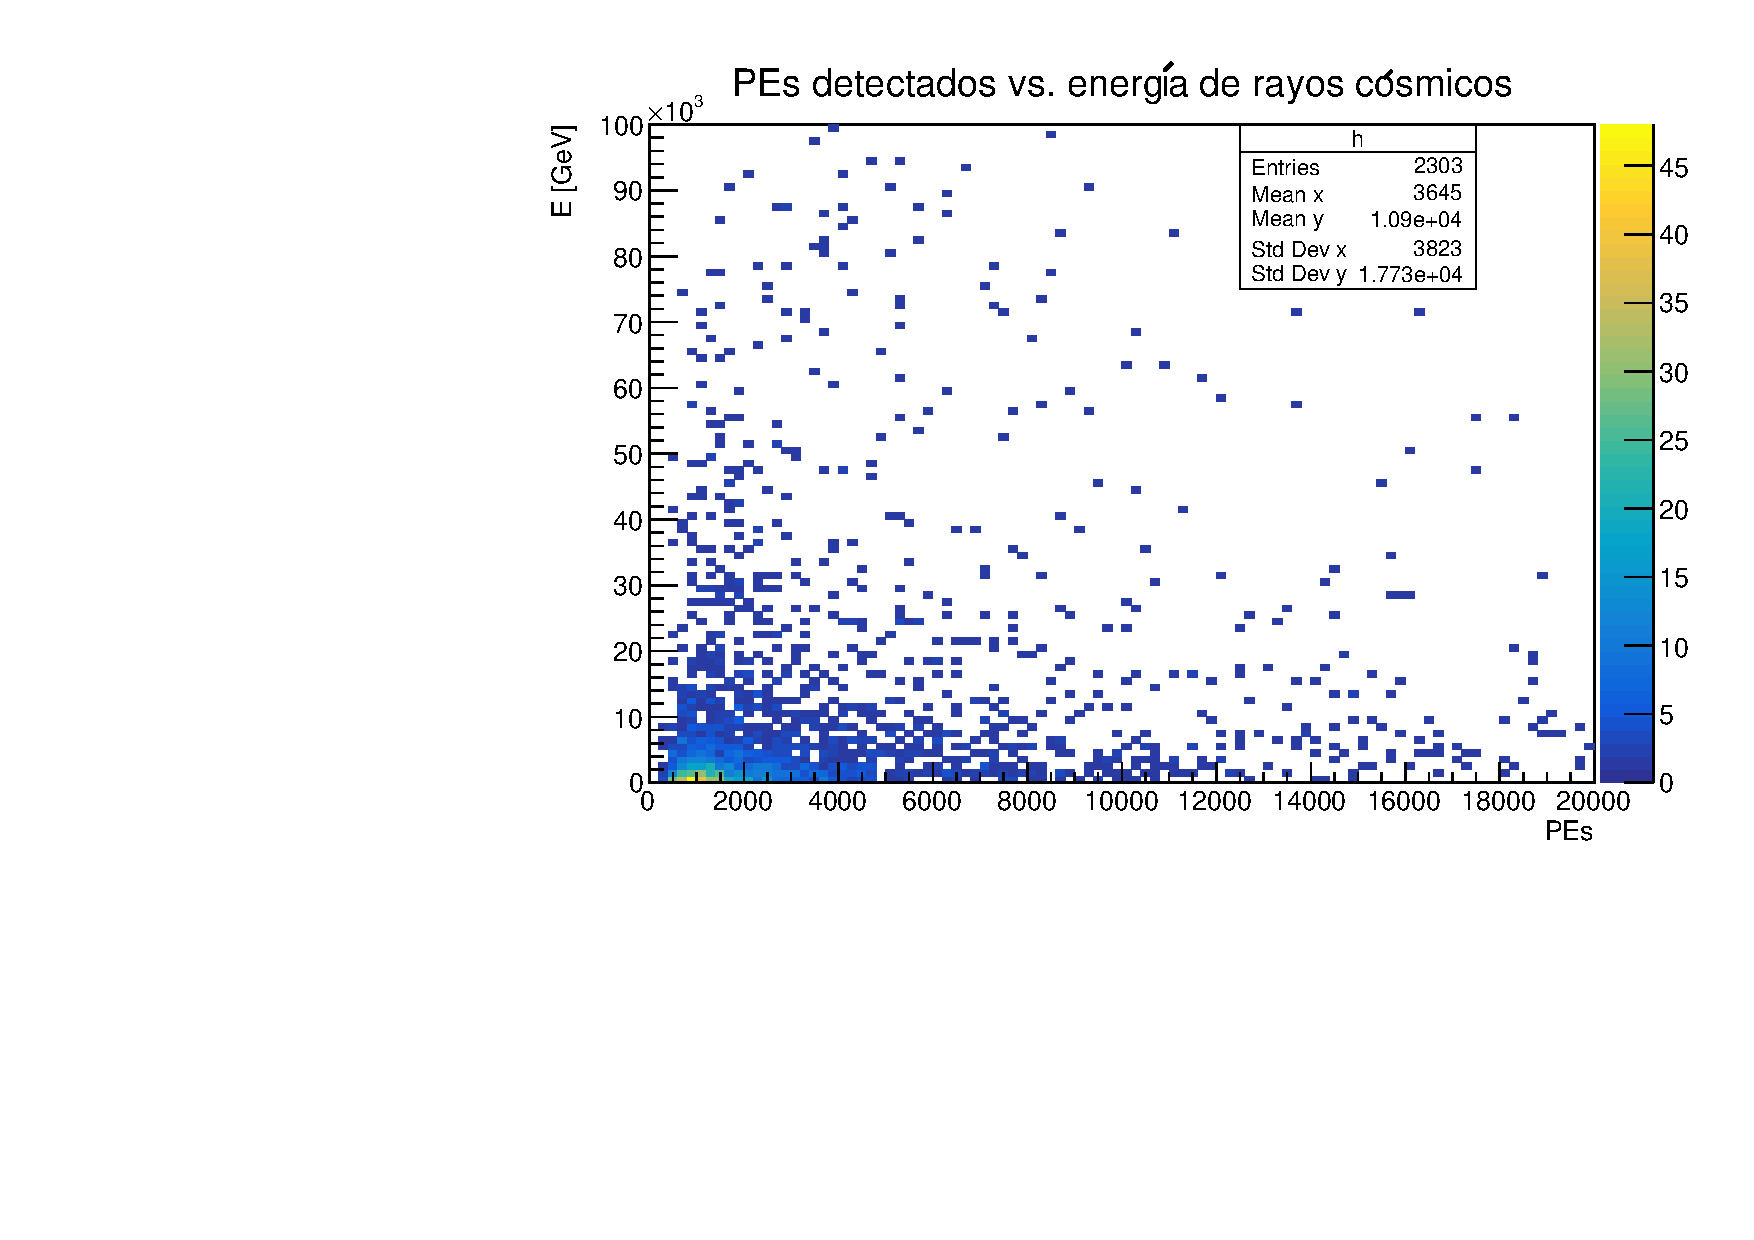
\includegraphics[width=1\textwidth]{../Figuras/Prob4A.pdf}
\caption{Número de PEs detectados vs. valor de la energía del rayo cósmico primario.}
\end{figure}




\end{document}